\documentclass[11pt,a4paper,english]{article} %document type and language
\usepackage[utf8]{inputenc}	% set character set to support some UTF-8
\usepackage{babel} 	% multi-language support
% \usepackage{sectsty}	% allow redefinition of section command formatting
\usepackage{tabularx}	% more table options
\usepackage{titling}	% allow redefinition of title formatting
\usepackage{imakeidx}	% create and index of words
\usepackage{xcolor}	% more color options
\usepackage{enumitem}	% more list formatting options
\usepackage{tocloft}	% redefine table of contents, new list like objects

\usepackage[centering,noheadfoot,margin=1in]{geometry}

%set TOC margins
\setlength{\cftbeforesecskip}{15pt} % skip in TOC

% remove paragraph white space and modify space between list items
\usepackage{parskip}

% Set font globally
\usepackage{lmodern}                % load Latin modern fonts
\usepackage[defaultsans]{cantarell} % cantarell fonts

% HACK: https://tex.stackexchange.com/questions/58087/how-to-remove-the-warnings-font-shape-ot1-cmss-m-n-in-size-4-not-available
\usepackage{anyfontsize}

% set LaTeX global font
\renewcommand{\familydefault}{\sfdefault}
\renewcommand{\sfdefault}{lmss}

% set styling headings
%\allsectionsfont{\usefont{OT1}{phi}{b}{n}}

\usepackage{float} 	% floats
\usepackage{graphicx}	% Graphics
\usepackage{amsmath}	% extensive math options
\usepackage{amssymb}	% special math symbols
\usepackage[Gray,squaren,thinqspace,thinspace]{SIunits} % elegant units
\usepackage{listings}                                   % source code

% Custom Operators
%% Expectation symbol
\DeclareMathOperator*{\E}{\mathbb{E}}
\DeclareMathOperator*{\Cov}{\mathrm{Cov}}
\DeclareMathOperator*{\Var}{\mathrm{Var}}

% missing math commands
\providecommand{\abs}[1]{\left\lvert#1\right\rvert}                    % |.|
\providecommand{\br}[1]{\left(#1\right)}                               % (.)
\providecommand{\sbr}[1]{\left[#1\right]}                              % [.]
\providecommand{\ddfrac}[2]{\frac{\displaystyle #1}{\displaystyle #2}}
% use \math rm{d} to include math differential

% independence symbol
% https://tex.stackexchange.com/questions/79434/double-perpendicular-symbol-for-independence
\newcommand{\indep}{\perp\!\!\!\!\perp}


% options for listings
\lstset{
  breaklines=true,
  postbreak=\raisebox{0ex}[0ex][0ex]{\ensuremath{\color{red}\hookrightarrow\space}},
  numbers=left,
  numbersep=5pt,
  numberstyle=\tiny\color{gray},
  basicstyle=\footnotesize\ttfamily
}

% NEEDS to be before hyperref, cleveref and autonum
% number figures, tables and equations within the sections
\numberwithin{equation}{section}
\numberwithin{figure}{section}
\numberwithin{table}{section}

% references and annotation, citations
\usepackage[small,bf,hang]{caption}        % captions
\usepackage{subcaption}                    % adds sub figure & sub caption
\usepackage{sidecap}                       % adds side captions
\usepackage{hyperref}                      % add hyperlinks to references
\usepackage[noabbrev,nameinlink]{cleveref} % better references than default~\ref
% Hack:https://tex.stackexchange.com/questions/285950/package-autonum-needs-the-obsolete-etex-package
\expandafter\def\csname ver@etex.sty\endcsname{3000/12/31}
\let\globcount\newcount
\usepackage{autonum}                       % only number referenced equations
\usepackage{url}                           % URLs
\usepackage{cite}                          % well formed numeric citations

% biblatex for references
% \usepackage{biblatex}
% \addbibresource{literature.bib}
% csquotes recommended: https://tex.stackexchange.com/questions/229638/package-biblatex-warning-babel-polyglossia-detected-but-csquotes-missing
% \usepackage{csquotes}

% format hyperlinks
\colorlet{linkcolour}{black}
\colorlet{urlcolour}{blue}
\hypersetup{colorlinks=true,
            linkcolor=linkcolour,
            citecolor=linkcolour,
            urlcolor=urlcolour}

%\usepackage{todonotes} % add to do notes
\usepackage{epstopdf}  % process eps-images
\usepackage{float}     % floats
\usepackage{fancyhdr}  % header and footer
% HACK: https://tex.stackexchange.com/questions/664532/fancyhr-warning-footskip-is-too-small
\setlength{\footskip}{14pt}

% default path for figures
\graphicspath{{figures/}}

% If we have multiple directories, specify them like this: \graphicspath{{figures_ch1/}{figures_ch2/}}.

% For rendering tikz
\usepackage{pgfplots}
\pgfplotsset{compat=1.18}
\usetikzlibrary{decorations.pathreplacing} % Load the library for drawing braces


% Define some math environments
\usepackage{amsthm}

\newtheorem{theorem}{Theorem}[section]
\newtheorem{corollary}{Corollary}[theorem]
\newtheorem{lemma}[theorem]{Lemma}

\theoremstyle{definition}
\newtheorem{definition}{Definition}[section]

\theoremstyle{remark}
\newtheorem*{remark}{Remark}

% set header and footer
\pagestyle{fancy}
\fancyhf{}                           % clear all header and footer fields
\cfoot{\thepage}                     % add page number
\renewcommand{\headrulewidth}{0pt} % add horizontal line of 0.4pt thick

\title{Inference in a Simple MTE Model}
\author{Julian Budde}
\date{\today}
\begin{document}
\maketitle
This document analyzes a simple version of the MTE model with a binary instrument and bounded outcome.
The goal is to extrapolate from a point-identified LATE for instrument-compliers to a larger sub-population.

I discuss solutions for constant splines, which in this case --- constant weights of target and identified parameters over a finite number of population intervals --- deliver sharp bounds (Theorem 4 in the paper).
The linear program in this simple example has analytical solutions which helps to illustrate the nature of the inference problem.

In particular, I discuss solutions in the cases of unrestricted MTR functions and under shape restrictions (e.g.\ increasing MTR functions).
In the first case, if the outcome is bounded between $0$ and $1$, the identified set is of the form
\begin{equation}
	\omega \beta_s \pm (1 - \omega),
\end{equation}
where both $\beta_s$ and $\omega$ are unknown and depend on the propensity score and the CEF of the outcome given the instrument.
In the second case, the solution to either the upper or the lower bound depends on whether the constraint is binding or not.
For example, with \textit{increasing} MTR functions, the solution to the upper bound is given by
\begin{equation}
	\overline{\beta^*}=
	\begin{cases}
		\omega \beta_s + (1 - \omega),& \quad \text{if } \beta_s \geq 0\\
		\beta_s + (1 - \omega),              & \quad \text{if } \beta_s < 0.
	\end{cases}
\end{equation}
This means that the upper bound is strictly smaller than the unrestricted bound stated above whenever $\beta_s$ is small enough.
With increasing MTRs the bound is attained by maximizing the MTR under treatment while leaving the MTR under no treatment unchanged.
If $\beta_s$ is negative, $1 \geq MTR^c_0 \geq MTR^c_1 \geq 0$ for the complier population, hence the unknown subpopulation cannot have a treament effect of $1$.

The next section formalizes the example.

\section{Simple Example: Extrapolating a LATE}
This section introduces the notation and setup considered here.
\subsection{Setup}
We consider a simple model with a binary instrument.
In this case we can identify a \textit{local} average treatment effect for the sub-population of instrument compliers.
Our goal is to extend this to a larger subpopulation.

The outcome is denoted $Y_i$ and has bounded support $[0,1]$ (without loss of generality).
The instrument $Z_i$ is binary.
Binary treatment $D_i$ is determined by the selection model with
\begin{equation}
	D_i = I\{p(Z_i) \geq U_i\},
\end{equation}
where $U_i\sim U(0,1)$, $U_i \indep Z_i$ and $I\{A\}$ denotes the indicator function for event $A$.
Thus, $p(z) \equiv P(D_i = 1 | Z_i = z)$ is the propensity score.

Assuming that it is known that $p(0) \leq p(1)$ we can identify $LATE(p(0), p(1))$, the local average treatment effect for the subpopulation with $U_i$ realizations in $\mathopen(p(0), p(1)\mathclose]$\footnote{In practice, it is unknown to the researcher whether $p(0) < p(1)$ and hence whether the target has upper bound $p(0) + \overline{u}$ or $p(1) + \overline{u}$. So probably the target should be treated as $\max\{p(1), p(0)\} + \overline{u}$ and the lower bound equivalently.}.
We are interested in extending this to $LATE(p(0), p(1) + \overline{u})$ with $\overline{u} \geq 0$ and such that $p(1) + \overline{u} \leq 1$.

In this simple case we can find an exact solution to the linear program presented in the previous section using a finite-dimensional approximation to the underlying MTR functions.
The reason --- as shown in the paper --- is that all weights, both for the identified and the target estimand, are constant over intervals of $u$.
In particular, partition $u\in[0,1]$ into the intervals $[0, p(0)], (p(0), p(1)], (p(1), \overline{u}], (\overline{u}, 1]$. Note that the relevant endpoints are the two propensity scores and the upper bound of the target parameter.

To approximate the underlying MTR functions for the non-parametric identified set we can simply use constant splines on each of the partitions, namely
\begin{align}
	I\{0 \leq u \leq p(0)\}, \\
	I\{p(0) < u \leq p(1)\}, \\
	I\{p(1) < u \leq \overline{u}\}, \\
	I\{\overline{u} < u \leq 1\}.
\end{align}

The weights on these splines are the choice variables of the linear program which can be stated as follows:
\begin{equation}
	[\text{Describe LP}].
\end{equation}

We have eight choice variables $\theta_{kd}$: One for each partition $k\in\{1,2,3,4\}$ and for each treatment state $d\in\{0,1\}$.
The choice variables in our setting are nuisance parameters.
We are solely interested in the upper and lower bound for the target parameter, that is the value of the linear program.


This linear program can easily be solved by hand and results in the following identified set:
\begin{equation}
	\beta^* \in [\omega\beta_s - (1 - \omega), \omega\beta_s + (1 - \omega)],
\end{equation}
where $\omega = \frac{p(1) - p(0)}{\overline{u} + p(1) - p(0)} = \frac{p(1) - p(0)}{\overline{u} + p(1) - p(0)}$.

This is intuitive: The target estimand is a weighted average of the identified $LATE(p(0), p(1))$ and the unknown $LATE(p(1), \overline{u})$.
The weights correspond to the relative size of the subpopulations and the bounds for the unknown LATE are $-1$ and $1$, respectively.
Importantly, this only holds because $LATE(p(0), p(1))$ does not put any restrictions on the MTR functions outside the interval $(p(0), p(1)]$, which is intuitive and can easily be seen from the LP constraints.
This is generally different for other identified target estimands like the OLS slope, which put non-zero weight outside this interval\footnote{OLS does so asymmetrically for $d=0$ and $d=1$ which reflects why OLS does not correspond to a well defined causal quantity in this model. Note: This would be interesting to connect to the ideas in~\cite{poirier2024quantifying}: How could we think about the subpopulation in terms of $u$?}.


Note that by the usual identification argument we have
\begin{equation}
	\beta_s = \frac{\E\left[Y|Z=1\right] - \E\left[Y|Z=0\right]}{p(1) - p(0)}.
\end{equation}
But this implies the interval simplifies to
\begin{equation}
	\beta^* \in \left[\frac{\E\left[Y|Z=1\right] - \E\left[Y|Z=0\right]}{\overline{u} + p(1) - p(0)} \pm (1 - \omega)\right].
\end{equation}

Now if $\overline{u}\geq0$ is fixed, this immediately tells we no longer have the weak identification problem when $p(1) - p(0)\geq0$ is close to zero. Further, in the case $p(1) - p(0) = 0$ we have that the numerator is also equal to zero by the exclusion restriction on $Z$. Hence, the identified set is --- obviously so --- given by $[-1, 1]$.

However, for asymptotics with \textit{both} $p(1) - p(0)$ and $\overline{u}$ going to zero with the sample size at the right rate issues with a denominator close to zero should again arise.

\subsection{Graphical Illustration}
Figure~\ref{fig:sm_upper_no_restr} illustrates the solution to the extrapolation problem for the upper bound.
First, note that the MTR functions outside $[p(0), p(1) + \overline{u}]$ are irrelevant as neither the identified nor the target parameter depends on them. Hence they are not depicted.
Next, note that in this special non-parametric case without any additional restrictions, the choices of $\theta_{2d}$ and $\theta_{3d}$ are independent.
Thus, the upper bound is given by any arguments that satisfy $\theta_{21} - \theta_{20} = \beta_s$ and the maximum upper bound is attained at $\beta_u = 1$ at $\theta_{31} = 1, \theta_{30} = 0$.
One such set of choice variables is depicted in the graph.

\begin{figure}
	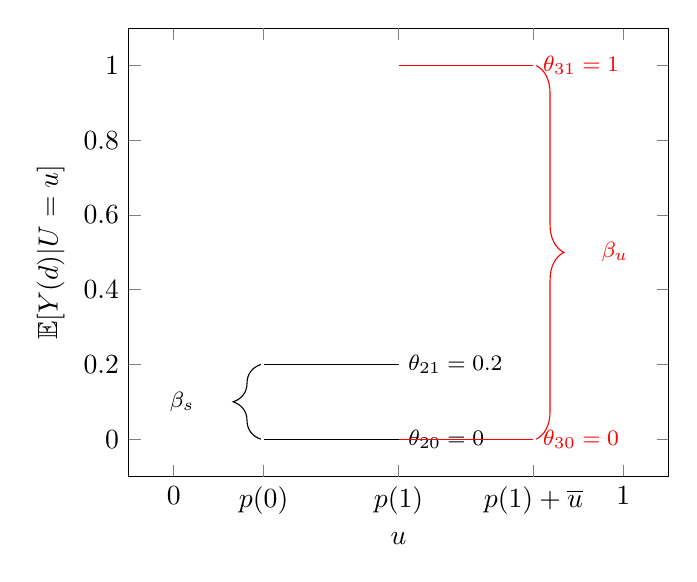
\begin{tikzpicture}
	\begin{axis}[
		xmin=-0.1, xmax=1.1,
		ymin=-0.1, ymax=1.1,
		xlabel=$u$,
		ylabel={$\E[Y(d)|U=u]$},
		xtick={0,1}, % Specify the x-axis ticks here
		extra x ticks={0.2, 0.5, 0.8}, % Specify the positions of the special x-axis ticks together
        extra x tick style={xticklabel style={color=black}}, % Apply a style to all extra x ticks
        extra x tick labels={$p(0)$, $p(1)$, $p(1) + \overline{u}$}, % Customize the labels of the special x-axis ticks
    ]

	\addplot [domain=0.2:0.5, color=black] {0} node[pos=1, right] {\footnotesize $\theta_{20} = 0$};
	\addplot [domain=0.2:0.5, color=black] {0.2} node[pos=1, right] {\footnotesize $\theta_{21} = 0.2$};

	\draw [decorate,decoration={brace,amplitude=10pt,raise=0pt},yshift=0pt, xshift=-1pt]
    (axis cs:0.2,0) -- (axis cs:0.2,0.2) node [black,midway,xshift=-1cm] {\footnotesize$\beta_s$};

	\addplot [domain=0.5:0.8, color=red] {0} node[pos=1, right, color=red] {\footnotesize $\theta_{30} = 0$};
	\addplot [domain=0.5:0.8, color=red] {1} node[pos=1, right, color=red] {\footnotesize $\theta_{31} = 1$};

	\draw [decorate,decoration={brace,amplitude=10pt,mirror,raise=0pt},yshift=0pt, xshift=1pt, color=red]
    (axis cs:0.8,0) -- (axis cs:0.8,1) node [red,midway,xshift=1cm] {\footnotesize$\beta_u$};


	\end{axis}
\end{tikzpicture}

	\caption{Solution for Upper Bound without Restrictions}\label{fig:sm_upper_no_restr}
\end{figure}

\subsection{Solutions with Restrictions}
\subsubsection{Monotone MTR Functions}
The first set of restrictions we consider are increasing MTR functions.
In terms of the program this corresponds to the following set of constraints:
\begin{equation}
	\theta_{k+1,d} \geq \theta_{k,d} \quad \text{for} \quad k \in \{2, 3, 4\} \text{ and } d \in \{0,1\}
\end{equation}

Under these additional restrictions the logic to attaining the upper bound is as follows:
We are only allowed to increase the MTR functions and $\beta_s$ is increasing in $\theta_{31}$ and decreasing in $\theta_{30}$.
Since both are constrained from below by $\theta_{21}$ and $\theta_{20}$ we make both as small as possible subject to $\theta_{21} - \theta_{20} = \beta_s$.
Then the has the feature $1 = \theta_{31} \geq \theta_{21}$ and $\theta_{30} = \theta_{20} \geq 0$.
To determine the remaining choice variables, differentiate between $\beta_s > 0$ and $\beta_s < 0$:
\begin{itemize}
	\item When $\beta_s > 0$ the constraint is \textit{not binding/redundant} (at least for the upper bound)\footnote{Technically it is binding but only since we have the general constraint $\theta_{kd} \geq 0$. In this sense it is redundant.}. Note that $\beta_s = \theta_{21} > \theta_{20} = 0$ is a possible solution satisfying the $\beta_s$ constraint.
	Hence, $1 = \theta_{31} > \theta_{30} = \theta_{20} = 0$ is a feasible solution implying $\beta_u = 1$. This is the upper bound without restrictions.
	\item When $\beta_s < 0$ the constraint will be \textit{binding}. The smallest set $\theta_{21}, \theta_{20}$ consistent with $\beta_s$ is given by $-\beta_s = \theta_{20} > \theta_{21} = 0$.
	Then the upper bound is attained by $1 = \theta_{31} > \theta_{30} = -\beta_s$ which results in $\beta_u = 1 + \beta_s < 1$. Thus, the constraint decreases the upper bound.
\end{itemize}

To summarize, the solutions to the upper and lower bound are given by the following function of $\beta_s$, which has a kink at $\beta_s = 0$:

\begin{equation}
	\overline{\beta^*}(\beta_s)=
	\begin{cases}
		\omega \beta_s + (1 - \omega),& \quad \text{if } \beta_s \geq 0\\
		\beta_s + (1 - \omega),              & \quad \text{if } \beta_s < 0,
	\end{cases}
\end{equation}
and
\begin{equation}
	\underline{\beta^*}(\beta_s)=
	\begin{cases}
		\beta_s - (1 - \omega),& \quad \text{if } \beta_s \geq 0\\
		\omega \beta_s - (1 - \omega),              & \quad \text{if } \beta_s < 0.
	\end{cases}
\end{equation}

Figure~\ref{fig:sm_upper_incr.tex} illustrates how the constraint is binding in the case with $\beta_s < 0$ for the upper bound.
Note we would like to set $\theta_{30} = 0$ but this violates the constraint $\theta_{30} \geq \theta_{20} = -\beta_s > 0$.

\begin{figure}
	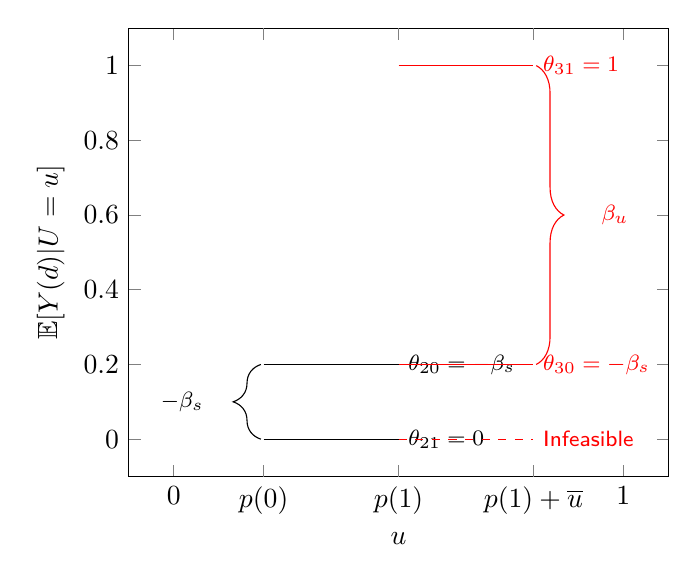
\begin{tikzpicture}
	\begin{axis}[
		xmin=-0.1, xmax=1.1,
		ymin=-0.1, ymax=1.1,
		xlabel=$u$,
		ylabel={$\E[Y(d)|U=u]$},
		xtick={0,1}, % Specify the x-axis ticks here
		extra x ticks={0.2, 0.5, 0.8}, % Specify the positions of the special x-axis ticks together
        extra x tick style={xticklabel style={color=black}}, % Apply a style to all extra x ticks
        extra x tick labels={$p(0)$, $p(1)$, $p(1) + \overline{u}$}, % Customize the labels of the special x-axis ticks
    ]

	\addplot [domain=0.2:0.5, color=black] {0.2} node[pos=1, right] {\footnotesize $\theta_{20} = -\beta_s$};
	\addplot [domain=0.2:0.5, color=black] {0} node[pos=1, right] {\footnotesize $\theta_{21} = 0$};

	\draw [decorate,decoration={brace,amplitude=10pt,raise=0pt},yshift=0pt, xshift=-1pt]
    (axis cs:0.2,0) -- (axis cs:0.2,0.2) node [black,midway,xshift=-1cm] {\footnotesize$-\beta_s$};

	\addplot [domain=0.5:0.8, color=red] {0.2} node[pos=1, right, color=red] {\footnotesize $\theta_{30} = -\beta_s$};
	\addplot [domain=0.5:0.8, color=red, dashed] {0} node[pos=1, right, color=red] {\footnotesize Infeasible};
	\addplot [domain=0.5:0.8, color=red] {1} node[pos=1, right, color=red] {\footnotesize $\theta_{31} = 1$};

	\draw [decorate,decoration={brace,amplitude=10pt,mirror,raise=0pt},yshift=0pt, xshift=1pt, color=red]
    (axis cs:0.8,0.2) -- (axis cs:0.8,1) node [red,midway,xshift=1cm] {\footnotesize$\beta_u$};


	\end{axis}
\end{tikzpicture}

	\caption{Upper Bound with Monotone MTR Functions}\label{fig:sm_upper_incr.tex}
\end{figure}

Figure~\ref{fig:sm_sol_upper} displays the solution to the upper bound $\overline{\beta^*}$ and lower bound $\underline{\beta^*}$ as a function of $\beta_s$ under different restrictions.
\begin{figure}
	\centering
	\begin{subfigure}{0.45\textwidth}
		\centering
		\begin{tikzpicture}
	\begin{axis}[
		xmin=-1.1, xmax=1.1,
		ymin=-1.1, ymax=1.1,
		xlabel=$\beta_s$,
		ylabel={$\overline{\beta^*}$},
		xtick={-1, 0, 1}, % Specify the x-axis ticks here
	    ytick={-1, 1},
        extra y ticks={-0.3, 0.7}, % Specify the positions of the special x-axis ticks together
        extra y tick style={yticklabel style={color=black}}, % Apply a style to all extra x ticks
        extra y tick labels={$-\omega$, $1-\omega$}, % Customize the labels of the special x-axis ticks
    ]

    % Unconstrained solution
	\addplot [domain=-1:1, color=black] {1-0.3 + 0.3*x};

    % Solution with monotonicity constraint
	\addplot [domain=-1:0, color=blue] {x + 0.7};
	\addplot [domain=0:1, color=blue] {0.3*x + 0.7};

    % Add text for each line
    \node at (axis cs:-0.25, -0.5) [color=black, anchor=west] {\footnotesize No Constraint};
    \node at (axis cs:-0.25, -0.75) [color=blue, anchor=west] {\footnotesize Increasing MTR Functions};

	\end{axis}
\end{tikzpicture}

		\caption{Solution to $\overline{\beta^*}$}
	\end{subfigure}
	\hfill
	\begin{subfigure}{0.45\textwidth}
		\centering
		\begin{tikzpicture}
	\begin{axis}[
		xmin=-1.1, xmax=1.1,
		ymin=-1.1, ymax=1.1,
		xlabel=$\beta_s$,
		ylabel={$\underline{\beta^*}$},
		xtick={-1, 0, 1}, % Specify the x-axis ticks here
	    ytick={-1, 1},
        extra y ticks={-0.7, 0.3}, % Specify the positions of the special x-axis ticks together
        extra y tick style={yticklabel style={color=black}}, % Apply a style to all extra x ticks
        extra y tick labels={$-(1-\omega)$, $\omega$}, % Customize the labels of the special x-axis ticks
    ]

    % Unconstrained solution
	\addplot [domain=-1:1, color=black] {0.3*x - (1-0.3)};

    % Solution with monotonicity constraint
	\addplot [domain=-1:0, color=blue] {0.3*x - (1-0.3)};
	\addplot [domain=0:1, color=blue] {x - (1-0.3)};

    % Add text for each line
    \node at (axis cs:-0.25, 0.75) [color=black, anchor=west] {\footnotesize No Constraint};
    \node at (axis cs:-0.25, 0.5) [color=blue, anchor=west] {\footnotesize Increasing MTR Functions};

	\end{axis}
\end{tikzpicture}

		\caption{Solution to $\underline{\beta^*}$}
	\end{subfigure}
	\caption{Solutions under Different Constraints}\label{fig:sm_sol_upper}
\end{figure}

\subsection{Estimation and Inference}
\paragraph{Unknown propensity score}
One subtle conceptual difficulty is that the researcher does not observe $p(0), p(1)$ but only a noisy estimate when they perform their extrapolation exercise. In terms of sampling, this would mean we over- or under-sample compliers, i.e.\ those with realizations $u_i\in (p(0), p(1)]$, resulting in a too large or too small difference in propensity scores.

We still consider the case where the researcher wants to perform inference on the parameter $p(0), p(1)$, which seems to be the only reasonable approach.

\paragraph{Plug-in Estimator}
The explicit solution above suggests a simple plug-in estimator for the identified set:
\begin{equation}
	\hat{\Theta}_0 = \left[\hat{\omega} \hat{\beta}^{LATE} - (1-\hat{\omega}), \hat{\omega}\hat{\beta}^{LATE} + (1-\hat{\omega}) \right].
\end{equation}
Here,
\begin{equation}
	\hat{\beta}^{LATE}  = \frac{1/N_1 \sum_{i=1}^N Z_i Y_i - 1/N_0 \sum_{i=1}^N(1-Z_i)Y_i}{1/N_1\sum_{i=1}^N Z_i D_i - 1/N_0\sum_{i=1}^N (1-Z_i)D_i}.
\end{equation}
where $N_1 = \sum_{i=1}^N Z_i$ and $N = N_0 + N_1$. Further,
\begin{equation}
	\hat{\omega} = \frac{\hat{p}(1) - \hat{p}(0)}{\overline{u} + \hat{p}(1) - \hat{p}(0)},
\end{equation}
where $\hat{p}(z)$ is an estimator of the propensity score.

Using the simplification noted above, the estimator can be equivalently written as
\begin{equation}
	.
\end{equation}


\bibliographystyle{plain}
\bibliography{refs.bib}

\end{document}
